\documentclass[spanish,a4paper]{article}

% Paquetes generales
\usepackage{ifthen}
\usepackage{amssymb}
\usepackage{amsmath}
\usepackage{multicol}
\usepackage[absolute]{textpos}
\usepackage{hyperref}
%\usepackage{graphicx}
\usepackage{caratula}

\setlength{\parindent}{12pt}

%% **************************************************************************
%
%  Package 'caratula', version 0.3 (para componer caratulas de TPs del DC).
%
%  CON MINIMAS MODIFICACIONES DEL TEAM ORGA2
%
%  En caso de dudas, problemas o sugerencias sobre este package escribir a
%  Brian J. Cardiff (bcardif arroba gmail.com).
%  Nico Rosner (nrosner arroba dc.uba.ar).
%
% **************************************************************************

% ----- Informacion sobre el package para el sistema -----------------------

\NeedsTeXFormat{LaTeX2e}
\ProvidesPackage{caratula}[2005/08/09 v0.3 Para componer caratulas de TPs del DC]
%\usepackage[pdftex]{graphicx}

% ----- Imprimir un mensajito al procesar un .tex que use este package -----

\typeout{Cargando package 'caratula' v0.3 (2005/08/09)}

% ----- Algunas variables --------------------------------------------------

\let\Materia\relax
\let\Submateria\relax
\let\Titulo\relax
\let\Subtitulo\relax
\let\Grupo\relax
\let\Fecha\relax
\let\Logoimagefile\relax

% ----- Comandos para que el usuario defina las variables ------------------

\def\materia#1{\def\Materia{#1}}
\def\submateria#1{\def\Submateria{#1}}
\def\titulo#1{\def\Titulo{#1}}
\def\subtitulo#1{\def\Subtitulo{#1}}
\def\grupo#1{\def\Grupo{#1}}
\def\fecha#1{\def\Fecha{#1}}
\def\logoimagefile#1{\def\Logoimagefile{#1}}

% ----- Token list para los integrantes ------------------------------------

\newtoks\intlist\intlist={}

% ----- Comando para que el usuario agregue integrantes --------------------

\def\integrante#1#2#3{\intlist=\expandafter{\the\intlist
    \rule{0pt}{1.2em}#1&#2&\tt #3\\[0.2em]}}

% ----- Macro para generar la tabla de integrantes -------------------------

\def\tablaints{%
    \begin{tabular}[t]{| l @{\hspace{4ex}} c @{\hspace{4ex}} l|}
        \hline
        \multicolumn{1}{|c}{\rule{0pt}{1.2em} Integrante} & LU &  \multicolumn{1}{c|}{Correo electr\'onico} \\[0.2em]
        \hline \hline
        \the\intlist
        \hline
    \end{tabular}}

% ----- Codigo para manejo de errores --------------------------------------

\def\se{\let\ifsetuperror\iftrue}
\def\ifsetuperror{%
    \let\ifsetuperror\iffalse
    \ifx\Materia\relax\se\errhelp={Te olvidaste de proveer una \materia{}.}\fi
    \ifx\Titulo\relax\se\errhelp={Te olvidaste de proveer un \titulo{}.}\fi
    \edef\mlist{\the\intlist}\ifx\mlist\empty\se%
    \errhelp={Tenes que proveer al menos un \integrante{nombre}{lu}{email}.}\fi
    \expandafter\ifsetuperror}


% ----- \maketitletxt correspondiente a la versión v0.2 (texto) ---------

\def\maketitletxt{%
    \ifsetuperror\errmessage{Faltan datos de la caratula! Ingresar 'h' para mas informacion.}\fi
    \thispagestyle{empty}
    \begin{center}
    \vspace*{\stretch{2}}
    {\LARGE\textbf{\Materia}}\\[1em]
    \ifx\Submateria\relax\else{\Large \Submateria}\\[0.5em]\fi
    \par\vspace{\stretch{1}}
    {\large Departamento de Computaci\'on}\\[0.5em]
    {\large Facultad de Ciencias Exactas y Naturales}\\[0.5em]
    {\large Universidad de Buenos Aires}
    \par\vspace{\stretch{3}}
    {\Large \textbf{\Titulo}}\\[0.8em]
    {\Large \Subtitulo}
    \par\vspace{\stretch{3}}
    \ifx\Grupo\relax\else\textbf{\Grupo}\par\bigskip\fi
    \tablaints
    \end{center}
    \vspace*{\stretch{3}}
    \newpage}

% ----- \maketitle correspondiente a la versión v0.3 (gráfica) -------------

\def\maketitlegraf{%
    \ifsetuperror\errmessage{Faltan datos de la caratula! Ingresar 'h' para mas informacion.}\fi
%
    \thispagestyle{empty}

    \ifx\Logoimagefile\relax\else\includegraphics{\Logoimagefile}\fi\hfill 
\includegraphics{imagenes/logodc.jpg}

    \vspace*{.12 \textheight}

    \noindent \textbf{\huge \Titulo}  \medskip \\
    \ifx\Subtitulo\relax\else\noindent\textbf{\large \Subtitulo} \\ \fi%
    \noindent \rule{\textwidth}{1 pt}

    {\noindent\large\Fecha \hspace*\fill \Materia} \\
    \ifx\Submateria\relax\else{\noindent \hspace*\fill \Submateria}\fi%

    \medskip%
    \begin{center}
        \ifx\Grupo\relax\else\textbf{\Grupo}\par\bigskip\fi
        \tablaints
    \end{center}%
    \vfill%
%
    \begin{minipage}[t]{\textwidth}
        \begin{minipage}[t]{.55 \textwidth}
            
\includegraphics{imagenes/logouba.jpg}
        \end{minipage}%%
        \begin{minipage}[b]{.50 \textwidth}
            \textbf{\textsf{Facultad de Ciencias Exactas y Naturales}} \\
            \textsf{Universidad de Buenos Aires} \\
            {\scriptsize %
            Ciudad Universitaria - (Pabell\'on I/Planta Baja) \\
                Intendente G\"uiraldes 2160 - C1428EGA \\
            Ciudad Aut\'onoma de Buenos Aires - Rep. Argentina \\
                Tel/Fax: (54 11) 4576-3359 \\
            http://www.fcen.uba.ar \\
            }
        \end{minipage}
    \end{minipage}%
%
    \newpage}

% ----- Reemplazamos el comando \maketitle de LaTeX con el nuestro ---------

\def\maketitle{\maketitlegraf}

\begin{document}

\titulo{Trabajo Pr\'{a}ctico}
\subtitulo{}

\fecha{\today}

\materia{Organizaci\'{o}n Del Computador 2}
\grupo{}

\integrante{Fosco, Martin Esteban}{449/13}{mfosco2005@yahoo.com.ar}
\integrante{Palladino, Juli\'{a}n}{231/13}{julianpalladino@hotmail.com}
\integrante{De Carli, Nicol\'{a}s}{164/13}{nikodecarli@gmail.com}

\maketitle

\section{Introducci\'{o}n}

Este Trabajo Pr\'{a}ctico se ha centrado en explorar el modelo de programaci\'{o}n \textbf{SIMD}, us\'{a}ndolo para una aplicaci\'{o}n popular del set de instrucciones SIMD de intel (SSE), procesamiento de im\'{a}genes y videos.\\
En particular, se implementaron 4 filtros de im\'{a}genes: Cropflip, Sierpinski, Bandas y Motion Blur.\\

Se ha buscado aprovechar los beneficios de SSE: 

\begin{itemize}

	\item Procesar conjuntos de datos de manera eficiente, ejecutando de manera paralela (al mismo tiempo) la misma instrucci\'{o}n sobre distintos datos.
	
	\item El uso de los registros XMM, los cuales proveen una gran versatilidad con la opci\'{o}n de ejecutar operaciones de punto flotante y enteras con distintas precisiones (sobre datos empaquetados o escalares).

	\item Minimizar los accesos a memoria.
	
	\item No se me ocurri\'{o} nada mas, pero llenen o borren, como les parezca mejor :)

\end{itemize} 
Luego de implementar en C y asm (procesando de manera escalar y vectorial los datos, respectivamente) los filtros de im\'{a}genes se ha comparado la performance de ambos modelos de programaci\'{o}n para determinar de manera aproximada la ventaja que se gana al trabajar sobre muchos datos de manera simult\'{a}nea.

\newpage

\section{Desarrollo}

\textbf{1.1)}\\

\noindent \textbf{a)}Al hacer el "objdump" no solo se imprime la funci\'{o}n "cropflip\_c.c", sino que tambi\'{e}n se imprimen varias funciones que utiliza GDB para hacer el debugging, tales como ".debug\_info", ".debug\_abbrev", ".debug\_aranges", etc. Tambi\'{e}n imprime ".comment" y "eh\_header", que contienen informaci\'{o}n sobre el Linker y el compilador.\\ \\
 \textbf{b)} Las variables locales las almacena en memoria, haciendo movs manualmente en el stack frame. (Por ej, poniendo las variables en [rbp-0x58], [rbp-0x60], [rbp-0x64]).\\ \\
 \textbf{c)} Se podr\'{i}a optimizar el almacenamiento de las variables locales. Como el acceso a memoria es mucho m\'{a}s ineficiente que el acceso a los registros, ser\'{i}a más \'{o}ptimo almacenar las variables en ellos. \\ \\ \\ \\

\noindent \textbf{1.2)}\\

\noindent \textbf{a)} -O1 no reduce mucho el tiempo de compilaci\'{o}n, y ejecuta una optimizaci\'{o}n "moderada". Se ve claramente que se reducen los accesos a memoria para las variables locales, y se reducen mucho las l\'{i}neas de c\'{o}digo.\\ \\
 \textbf{b)} Usando otros par\'{a}metros como -O2 u -O3 se hace la compilaci\'{o}n con más optimizaciones cuanto más grande sea el n\'{u}mero. Tambi\'{e}n est\'{a}n -Os que optimiza el tama\~{n}o del c\'{o}digo y -Og que optimiza el debugging.\\ \\



\noindent \textbf{c)}\\

\begin{itemize}

	\item \textbf{FDCE:} Hace eliminaci\'{o}n de "dead code" (C\'{o}digo muerto), es decir, borra el c\'{o}digo que consume recursos pero sus resultados nunca son utilizados.
	\item \textbf{FDSE:} Hace eliminaci\'{o}n de "dead store" (Almacenamiento muerto), o sea, ignora aquellas variables que despu\'{e}s no llegan a ser utilizadas. 
	\item \textbf{-fif-conversion y -fif-conversion2:} Reemplazan condicionales por equivalentes aritm\'{e}ticos. Esto incluye funciones como movimientos condicionales, m\'{i}nimos, m\'{a}ximos, funci\'{o}n "abs", entre otros. Luego de ver los resultados del experimento 3.1 (Saltos condicionales en el filtro Bandas) queda claro que esta optimizaci\'{o}n es extremadamente \'{u}til.

\end{itemize}

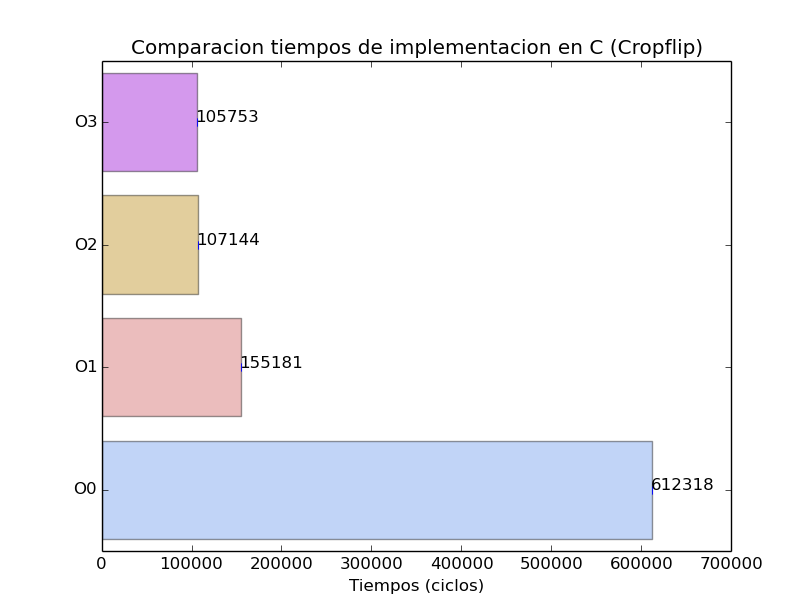
\includegraphics[width=350pt]{cropCompC.png}
En el gr\'{a}fico se nota la clara diferencia entre las corridas con optimizaciones y sin ellas. El criterio fue el mismo que aplicamos en los experimentos de m\'{a}s adelante (Haciendo 1000 iteraciones).

\newpage

\textbf{1.3)}\\ \\ 
En este experimento consideraremos diferentes criterios realizando siempre 10 mediciones, con outliers, sin ellos, y agregando programas en C++ que trabajen en simult\'{a}neo.\\ \\

\noindent \textbf{a)} \indent \textbf{Resultados:}\\ \\ 422861, 242136, 186857,\\ 194709, 234097, 221979,\\ 247912, 227976, 223245,\\ 200770.\\ \\ \\

\noindent\textbf{b)} \indent \textbf{Resultados:}\\ \\ 289209, 302654, 258757,\\ 254428, 248527, 254606,\\ 260391, 338981, 373612,\\ 280937 \\ \\ \\

\noindent \textbf{c)} \\ \textbf{10 mediciones}\\Esperanza: 240254.2  Desv\'{i}o standard: 67250.78758  Varianza: 4522668429.51111\\
\noindent \textbf{10 mediciones con el programa en simult\'{a}neo:}\\Esperanza: 286210.2  Desv\'{i}o standard: 41607.01932
Varianza: 1731144056.62222\\ \\ \\
\textbf{d)} \textbf{10 mediciones sin 2 outliers:}\\Esperanza: 224103  Desv\'{i}o standard: 18595.78063  Varianza: 345803057.14286\\ \\ \\

\textbf{e)} \\ INSERT GRAFICOU HERE \\ \\ \\

\newpage

\textbf{1.4)}\\ \\

\indent \textbf{C O0-} 613445 ciclos\\
\indent \textbf{C O1-} 156148 ciclos\\
\indent \textbf{C O2-} 106859 ciclos\\
\indent \textbf{C O3-} 106740 ciclos\\

\textbf{asm-} 46671\\ \\ \\

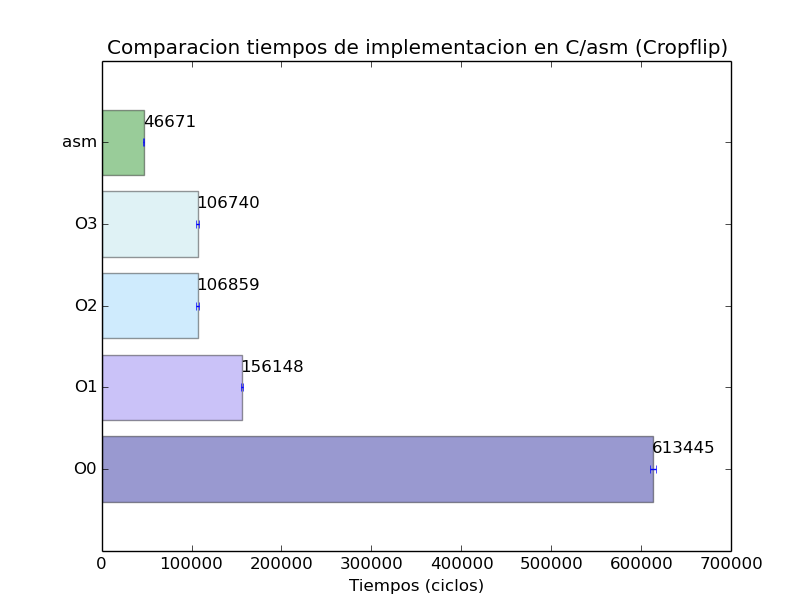
\includegraphics[width=330pt]{CompCasm1.png}

\newpage



\section{Conclusi\'{o}n}



\end{document}
